\chapter{Criptografia Moderna}
\label{cha:criptografia-moderna}

No final dos anos 40, com o desenvolvimento dos primeiros computadores e a experiência da quebra das cifras mecanicamente produzidas por poderosas máquinas desenvolvidas pelo esforço de guerra do nazismo, alguns cientistas se voltaram para um problema central no campo da criptografia: o que torna um sistema de criptografia seguro?

As cifras que vimos até agora são conhecidas como {\em cifras clássicas} exatamente porque elas precedem esse debate moderno, e não é à toa que foram todas derrotadas cedo ou tarde.
Informalmente, poderíamos dizer que o problema dos esquemas clássicos de criptografia é que eles mantêm muita informação sobre a mensagem original, como a frequência das letras, dos dígrafos, letras duplas, entre outros.
Esses padrões permitem que criptanalistas descubram o texto original sem conhecer a chave.

Não é uma coincidência, portanto, que a primeira tentativa de formalizar o conceito de segurança tenha sido proposta por Claude Shannon, o fundador da teoria da informação.
Shannon introduziu conceitos fundamentais que ajudaram a definir o que faz um sistema de criptografia ser verdadeiramente seguro.
Sua abordagem foi a base para o desenvolvimento de métodos mais robustos e seguros de criptografia.

\section{Sigilo Perfeito}
\label{sec:sigilo-perfeito}

Shannon definiu o que hoje chamamos de sigilo perfeito.
Um sistema de criptografia garante o {\em sigilo perfeito} se a probabilidade da mensagem original for independente da probabilidade da cifra.

Vamos relembrar o que são eventos independentes.
A probabilidade da mensagem original ser $m$ dado que a cifra é $c$ deve ser igual à probabilidade da mensagem ser $m$ independentemente da cifra.
Em termos matemáticos, isso significa que:

\begin{displaymath}
  Pr[M = m | C = c] = Pr[M = m]
\end{displaymath}

É nesse sentido preciso que dizemos que a cifra $c$ não guarda nenhuma informação sobre a mensagem $m$.
Quando essa condição é satisfeita, mesmo que um interceptador obtenha a cifra $c$, ele não obtém nenhuma pista sobre qual era a mensagem $m$.
Todas as mensagens possíveis são igualmente prováveis, tornando a criptoanálise impossível.
Ou seja, podemos dizer que um sistema de criptografia garante o sigilo perfeito se as cifras produzidas por ele não guardam informação da mensagem original.

De forma equivalente, um sistema de criptografia garante o sigilo perfeito se uma cifra $c$ qualquer pode ter sido produzida com igual probabilidade por qualquer mensagem $m$.
Dada uma cifra $c$ e duas mensagens $m_1$ e $m_2$ quaisquer, temos que:

\begin{displaymath}
  Pr[C = c | M = m_0] = Pr[C = c | M = m_1]
\end{displaymath}


A cifra de substituição não garante o sigilo perfeito. Vamos ver um exemplo simples que mostra isso.

Suponha que nossa cifra é {\tt OVO}.
Vamos calcular a probabilidade de diferentes mensagens originais terem gerado essa cifra.

Se a mensagem original for {\tt ana}, e usamos uma cifra de substituição específica que mapeia {\tt a} para {\tt O} e {\tt n} para {\tt V}, a mensagem cifrada resultante seria {\tt OVO}.
Se a chave, que nesse caso é uma permutação, foi escolhida de forma aleatória, temos 1 chance em 23 que a letra {\tt a} da mensagem original tenha sido substituída por {\tt O} na cifra.
A chance de {\tt n} ser substituído por {\tt V} é então 1 em 22, porque {\tt n} não pode ser substituído por {\tt O} que já foi escolhido.
Portanto, a probabilidade da mensagem original {\tt ana} gerar a cifra {\tt OVO} é $\frac{1}{22.23} = \frac{1}{650}$.

Agora, considere outra mensagem possível, como {\tt eva}.
Se a letra {\tt e} fosse substituída por {\tt O}, isso não seria possível porque {\tt a} também precisaria ser substituída por {\tt O}.
No entanto, na cifra de substituição, uma letra só pode ser mapeada para uma outra única letra, não duas vezes para a mesma letra.
Portanto, a probabilidade de a mensagem original ser {\tt eva} e gerar a cifra {\tt OVO} é 0.

Esse exemplo simples demonstra que as mensagens originais {\tt ana} e {\tt eva} têm probabilidades diferentes de gerar a cifra {\tt OVO}.
Em outras palavras, a cifra de substituição não garante o sigilo perfeito, pois a probabilidade da cifra ser gerada não é independente da mensagem original.
Portanto, algumas mensagens têm uma probabilidade maior de gerar uma cifra específica do que outras, o que pode fornecer pistas para a criptoanálise.

Outra forma de definir o sigilo perfeito é por meio de um jogo entre o sistema de criptografia $\Pi = \langle Gen, E, d \rangle$ e um adversário $\mathcal{A}$ que quer decifrá-lo.
O jogo funciona da seguinte maneira:

\begin{enumerate}
\item O adversário ($\mathcal{A}$) escolhe duas mensagens quaisquer $m_0$ e $m_1$.
  A única restrição é que elas devem ter o mesmo tamanho.
  O adversário então envia essas duas mensagens para o sistema $\Pi$.
\item O sistema então sorteia uma chave $k$ usando o algoritmo $Gen$ e escolhe aleatoriamente uma das duas mensagens.
\item O sistema criptografa a mensagem escolhida com a chave gerada  ($E(k,m) = c$) e devolve a cifra resultante $c$ para o adversário.
\item O adversário pode utilizar todos os meios ao seu dispor para descobrir qual das duas mensagens foi criptografada.
\end{enumerate}

Um sistema de criptografia garante o sigilo perfeito se, ao final do jogo, o adversário não tiver nenhuma vantagem em descobrir qual mensagem foi criptografada.

\begin{center}
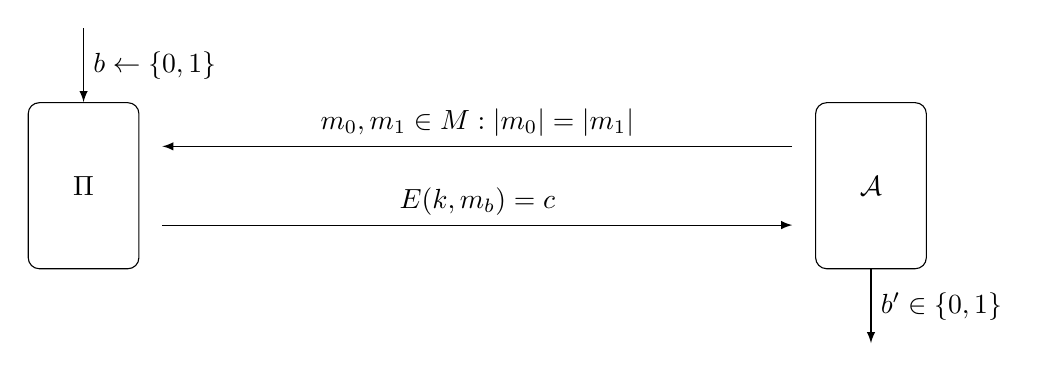
\begin{tikzpicture}[node distance=2cm,auto,>=latex]
\tikzset{
  player/.style={draw,shape=rectangle,rounded corners,minimum width=4em,minimum height=6em}
}
\node[player] (system) {$\Pi$};
\node[player] (adversary) at (10,0) {$\mathcal{A}$};
\draw[->] (9,.5) -> node[above]{$m_0, m_1 \in M : |m_0| = |m_1|$} (1,.5);
\draw[->] (1,-.5) -> node[above]{$E(k,m_b) = c$} (9,-.5);
\draw[->] (0,2) -> node{$b \leftarrow \{0,1\}$} (system);
\draw[->] (adversary) -> node{$b' \in \{0,1\}$} (10,-2);
\end{tikzpicture}
\end{center}

Note que mesmo sem nenhuma informação, o adversário pode acertar qual das duas mensagens foi cifrada com $50\%$ de probabilidade, simplesmente chutando uma das duas.
O sistema $\Pi$ garante sigilo perfeito se isso for o melhor que o adversário pode fazer.
Ou seja, se a probabilidade de que ele vença o jogo for exatamente $\frac{1}{2}$


\section{One Time Pad}
\label{sec:otp}

Temos agora uma definição formal de segurança.
Vimos que a cifra de substituição não satisfaz essa definição, mas na verdade nenhuma das cifras clássicas a satisfaz.
Não seria desejável que essas cifras satisfizessem a definição, pois vimos no capítulo anterior que nenhuma das cifras clássicas é segura e todas podem ser derrotadas se o adversário tiver acesso a uma cifra de tamanho suficientemente grande.
Ficamos então com o desafio de encontrar algum sistema que satisfaça essa definição, caso tal sistema exista.

No que segue, apresentaremos um sistema chamado {\em One Time Pad} (OTP), também conhecido como {\em cifra de Vernan}, e mostraremos que ele garante o sigilo perfeito.
A partir deste ponto, conforme começarmos a investigar sistemas a serem implementados computacionalmente, consideraremos que o espaço $M$ das mensagens (assim como o espaço $C$ das cifras) será representado como sequências de bits.
No caso específico do OTP assumiremos que as mensagens e a cifras possuem um tamanho fixo $n$.
Mais importante é o fato de que o universo das chaves é também um conjunto de sequências de bits do mesmo tamanho.
Assim temos que $M = C = K = \{0,1\}^n$.
O sistema $\Pi = \langle Gen, E, D \rangle$ é definido pelos seguintes algoritmos:
\begin{itemize}
\item $Gen := k \leftarrow \{0,1\}^n$
\item $E(k,m) = [m_0 + k_0\ mod\ 2] \dots [m_n + k_n\ mod\ 2] = m \xor k$
\item $D(k,c) = [c_0 + k_0\ mod\ 2] \dots [c_n + k_n\ mod\ 2] = c \xor k$
\end{itemize}

Para verificar a corretude do sistema basta notar que:

\begin{eqnarray*}
  D(k, E(k, m)) & = & D(k, k \xor m)\\
                & = & k \xor (k \xor m)\\
                & = & (k \xor k) \xor m\\
                & = & m
\end{eqnarray*}

A derivação usa o fato de que a operação de {\em ou exclusivo} $\xor$ é associativa, que $x \xor x = 1$ e $1 \xor x = x$ para todo sequência de bits $x \in \{0,1\}^*$.
Deixamos como exercício mostrar essas três propriedades da operação.

\begin{example}
  Considere uma mensagem $m = 101010$ e uma chave $k = 010001$.
Usando o sistema One Time Pad a cifra produzida é a seguite:

\begin{displaymath}
  \begin{array}{ccccc}
    m & \xor & k & = & c \\
    101010 & \xor & 010001 & = & 111011
  \end{array}
\end{displaymath}
\end{example}

Como antecipado, é possível, e relativamente simples provar que o OTP possui sigilo perfeito.

\begin{theorem}
  O sistema de criptografia {\em One Time Pad} possui sigilo perfeito.
\end{theorem}

\begin{proof}
  Seja $K = M = C = \{0,1\}^n$.
  Dada uma cifra $c \in C$ e uma mensagem qualquer $m \in M$, existe uma única chave $k \in K$ tal que $E(k,m) = c$.
  A chave é exatamente $k = m \xor c$, pois:

  \begin{eqnarray*}
    E(k, m) & = & k \xor m \\
            & = & (m \xor c) \xor m\\
            & = & (m \xor m) \xor c\\
            & = & c
  \end{eqnarray*}

Como existe exatamente uma chave possível que faz com que $E(k,m) = c$, temos que a probabilidade de se produzir $c$ dado uma mensagem qualquer $m$ é igual a probabilidade de sortear uma chave específica no universo $K = \{0,1\}^n$ que é $\frac{1}{2^n}$:
\begin{displaymath}
  Pr[C = c | M = c] = \frac{1}{2^n}
\end{displaymath}

Essa probabilidade é idêntica para qualquer $m \in M$.
Portanto, temos que $Pr[C = c| M = m_0] = Pr[C = c | M = m_1] = \frac{1}{2^n}$.
\end{proof}

O {\em One Time Pad} possui duas severas limitações.
A primeira é indicada pelo próprio nome do sistema.
O sistema supõe que a chave de criptografia $k$ seja usada exatamente uma vez (``one time'').
Caso a mesma chave $k$ seja usada para criptografar duas mensagens distintas $m_1$ e $m_2$, o sistema se torna completamente inseguro.

Para ilustrar essa limitação considere que duas cifras $c_0$ e $c_1$ foram produzidas usando a mesma chave $k$.
Assim temos que $c_0 = k \xor m_0$ e $c_1 = k \xor m_1$.
Note o que acontece quando aplicamos o ou exclusivo entre as duas cifras eliminamos a chave:


\begin{eqnarray*}
  c_0 \xor c_1 & = & (k \xor m_0) \xor (k \xor m_1)\\
              & = & (k \xor k) \xor (m_0 \xor m_1)\\
              & = & m_0 \xor m_1
\end{eqnarray*}

Uma vez eliminada a chave, é fácil separar as mensagens $m_0$ de $m_1$ utilizando uma técnica similar ao ataque de frequência.

A segunda e mais crítica limitação do OTP é o tamanho de sua chave.
A suposição que fizemos é que o tamanho da chave deve ser tão grande quanto a mensagem a ser cifrada.
Há uma série de problemas práticos com isso.
Computacionalmente não é possível gerar chaves aleatórias muito grandes, o que limita o tamanho das mensagens que podemos cifrar.
Além disso, assumimos que as chaves são compartilhadas entre as partes.
Deixamos os detalhes sobre a distribuição de chaves para o Capítulo \ref{cha:distribuicao-chaves}, mas por ora podemos adiantar que se nossa chave é tão grande quanto a mensagem, porque não enviamos a mensagem pelo mesmo canal que enviaríamos a chave?
Enfim, um sistema cuja a chave seja tão grande quanto a mensagem é de muito pouca utilidade prática.

Encerramos este capítulo mostrando que esta segunda limitação do OTP infelizmente não é uma peculiaridade do sistema.
Na verdade todo sistema que possua sigilo perfeito está fadado a ter chaves tão grandes ou maiores do que a mensagem.
Esse resultado negativo foi proposto e demonstrado pelo próprio Shannon ainda nos anos 40.


\begin{theorem}[Shannon]
Seja $\Pi = \langle Gen, E, D \rangle$ um sistema que garante o sigilo perfeito, então temos que $|K| \geq |M|$.
\end{theorem}
\begin{proof}
  Consideraremos $M(c)$ como o conjuto de todas as mensagens que podem produzir $c$, ou seja, as mensagens $m \in M$ tal que $E(k, m) = c$ para algum $k \in K$.
  Se existissem $m' \neq m''$ tais que $E(k, m') = E(k, m'') = c$ então $\Pi$ não poderia ser correto, pois $D(k, c)$ não poder ser $m'$ e $m''$ ao mesmo tempo.
  Portanto o número de mensagens que podem ser cifradas como $c$ é menor ou igual ao número de chaves, ou em símbolos, $|M(c)| \leq |K|$.
  Agora suponha por absurdo que $|K| < |M|$.
  Neste caso existiria uma mensagem $m \notin M(c)$ e, portanto, $Pr[M = m] \neq 0$.
  Mas, por definição, temos que $Pr[C = c | M = m] = 0$ contradizendo a hipótese deu que $\Pi$ garante o sigilo perfeito.
\end{proof}

A definição de Shannon foi a primeira tentativa séria de definir segurança de sistemas de criptografia, mas o próprio autor da definição foi capaz de demonstrar suas limitações.
Nos próximos capítulos apresentaremos definições de segurança mais fracas e mais úteis para nossos propósitos.

A definição, proposta por Shannon, estabelece que um sistema garante o {\em sigilo perfeito} se a cifra não guarda nenhuma informação da mensagem que a produziu.
No final do capítulo, porém, vimos que esta definição não é muito útil na prática, pois obriga o universo de chaves a ser pelo menos tão grande quanto o universo das mensagens.

Apesar do fracasso desta primeira tentativa de formalizar o conceito de segurança, não abandonaremos a ideia geral.
A abordagem da {\em criptografia moderna} \cite{Goldwasser84}, que utilizaremos nesta apostila, segue três princípios básicos:
\begin{enumerate}
\item {\em definições formais:} As noções de segurança utilizadas serão apresentadas de maneira formal por meio de definições.
As definições prévias nos ajudam a comparar sistemas e avaliar sua segurança a partir de critérios estabelecidos previamente.
\item {\em suposições explícitas:} Na maioria dos casos seremos forçados a fazer suposições sobre os sistemas de criptografia que não seremos capazes de demonstrar.
Ainda assim, é imprescindível explicitar essas suposições de maneira clara e formal.
Nossa incapassidade de provar tais suposições não nos impede de validá-las empiricamente.
Grande parte do trabalho envolvido na criptografia moderna consiste em validar testar as suposições sobre um sistema e buscar suposições mais simples e básicas.
\item {\em demonstrações formais:} Quando somos capazes de formalizar nossas suposições e a definição de segurança desejada, eventualmente podemos demonstrar que um sistema que satisfaz as suposições garante determinada noção de segurança.
Esse tipo de demonstração reduz o problema da segurança às suposições do sistema que devem ser mais simples e mais fáceis de validar empiricamente.
Esta redução permite que se substitua um sistema cuja suposição foi falseada antes que ele seja quebrado.
\end{enumerate}

As definições de segurança em geral possuem dois componentes: uma garantia de segurança -- o que pode ser considerado um ataque bem sucedido -- e um modelo de ameaças.
Por exemplo, na definição de {\em sigilo perfeito} a garantia de segurança é que nenhuma informação sobre a mensagem esteja contida na cifra -- ou como formulamos, a probabilidade de ocorrência da cifra deve ser independente da probabilidade de ocorrência da mensagem -- e o modelo de ameaça assume que o adversário tem acesso apenas ao texto cifrado e nada mais.
Os modelos de ameaças que estudaremos no livros incluem:
\begin{itemize}
\item {\em ataque ciphertext-only:} Este é o modelo assumido na definição de sigilo perfeito.
Nele assumimos que o adversário tem acesso apenas a um texto cifrado de tamanho arbitrário.
\item {\em ataque chosen-plaintext:} Neste modelo, além de assumir que o adversário tem acesso à cifra, assumimos que ele é capaz de escolher uma quantidade de mensagens e verificar como elas seriam cifradas pelo sistema.
\item {\em ataque chosen-ciphertext:} Neste modelo assumimos que o adversário é também capaz de escolher certas cifras e verificar como elas seriam decifras pelo sistema.
\end{itemize}

Essas definições são progressivamente mais fortes, ou seja, assumem progressivamente maior capacidade de ataque do adversário.
Note que nossos modelos de ataque não fazem qualquer suposição sobre a estratégia utilizada pelo adversário.
Em geral, a definição mais adequada depende das necessidades do problema em mãos -- eventualmente pode ser desejável um sistema mais fraco e mais eficiente.

Nossa primeira tentativa de definir segurança esbarrou na limitação inconveniente expressa pelo teorema de Shannon.
Afirmamos no capítulo anterior que o sigilo perfeito pode ser definido por meio de um jogo.
O sigilo perfeito é garantido se nenhum adversário for capaz de distinguir qual mensagem foi encriptada pelo sistema.
Para contornar as limitações expressas pelo teorema de Shannon, enfraqueceremos este tipo de definição de duas formas:
\begin{itemize}
\item O adversário deve ser {\em eficiente} e usar sua estratégia em um tempo razoável.
  Ou seja, eventualmente um adversário pode derrotar o sistema desde que seja dado a ele tempo suficiente.
  A existência de um adversário como este não violará nossa definição de segurança, pois não traz uma real ameaça na prática.
\item O adversário pode eventualmente derrotar o sistema, mas com uma {\em probabilidade muito pequena}.
Colocado de outra maneira, a cifra pode guardar alguma informação sobre a mensagem desde que seja muito pouca.
\end{itemize}

\section{Abordagem Assintótica}
\label{sec:abord-assint}

Em termos práticos o que buscamos uma noção de segurança em que para um adversário ter sucesso ele precisaria rodar seu algoritmo em uma máquina excelente por um intervalo bem grande de tempo.
Alternativamente esperamos que eventualmente o adversário derrote o sistema em pouco tempo, mas com uma probabilidade muito baixa.
O problema com essa abordagem é como definir o que seria uma ``máquina excelente'', um ``intervalo bem grande de tempo'' e uma ``probabilidade muito baixa''.
Essas questões são particularmente complicados em um contexto em que a capacidade computacional evolui de maneira acelerada.

Ao invés de estabelecer valores fixos para definir esses limites, partiremos de uma {\em abordagem assintótica}.
Suporemos que o algoritmo de geração de chaves $Gen$ recebe um {\em parâmetro de segurança} $n$ e estabeleceremos nossos limites em função deste parâmetro -- tipicamente denotaremos esse valor usando a notação unária $1^n$, pois a tempo de execução costuma ser calculado como uma função do tamanho da entrada.
Para os efeitos desta apostila podemos assumir que o parâmetro está relacionado ao tamanho da chave a ser gerada e que é de conhecimento público.
O parâmetro de segurânça permite que as partes ajustem seu sistema para o nível desejado de segurança -- aumentar seu tamanho costuma refletir em um aumento no tempo de processamento do sistema e em um aumento no tamanho da chave, portanto, quem projeta o sistema tem um incentivo para querer minimizá-lo as custas de diminuir sua segurança.
A capacidade de ajustar o parâmetro de segurânça possui grandes vantagens práticas, pois permite se defender de adversários com poder computacional mais forte com o passar do tempo.

Vamos estabelecer que o adversário buscará quebrar a cifra usando um algorítmo randomizado polinomial em $n$ e que ele pode vencer com uma probabilidade desprezível em $n$.
A suposição de que o adversário usa um algoritmos randomizado é forte, significa que ele é capaz de acessar uma quantidade arbitrária de bits aleatórios.
Isso certamente não é possível na prática, mas serve bem aos propósitos de uma análise de pior caso.
Já a probabilidade ser {\em desprezível} significa que ela cresce assintoticamente mais devagar do que o inverso de qualquer polinômio.
Formalmente, $\varepsilon: \mathbb{N} \to \mathbb{N}$ é {\em desprezível} se para todo polinômio $p$ existe um número positivo $N$ tal que para todo $n > N$ temos que $\varepsilon(n) < \frac{1}{p(n)}$.

Estamos agora em condições de reescrever a definição de segurança formalmente incorporando os enfraquecimentos descritos neste capítulo.

\begin{definition}
  Considere o jogo apresentado no Capítulo \ref{cha:sigilo-perfeito}, um sistema $\Pi = \langle Gen, E, D \rangle$ é seguro contra ataques {\em ciphertext-only} se para todo adversário polinomial $\mathcal{A}$ existe uma função desprezível $\varepsilon$ tal que para todo $n$:
\begin{displaymath}
  Pr[PrivK^{eav}_{\Pi, \mathcal{A}}(n) = 1] \leq \frac{1}{2} + \varepsilon(n)
\end{displaymath}
\end{definition}

Lembrando que agora o algoritmo $Gen$ recebe como o parâmetro de segurança $n$ em notação unária para gerar a chave de tamanho apropriado.
Em palavras, a definição estabelece que um sistema é seguro contra ataques {\em ciphertext-only} se nenhum algoritmo eficiente é capaz de derrotá-lo com probabilidade consideravelmente maior do que $\frac{1}{2}$.
Resta mostrar um sistema que satisfaça essa definição.


\section{Exercícios}
\label{sec:exercicios}

\begin{exercicio}
  Mostre que o $0$ é elementro neutro na operação $\xor$, ou seja, que para todo $x \in \{0,1\}^*$ temos que $x \xor 0 = 0 \xor x = x$.
\end{exercicio}

\begin{exercicio}
  Mostre que a operação $\xor$ é {\em associativa}, ou seja, que para todo $x,y,z \in \{0,1\}^*$ temos que $x \xor (y \xor z) = (x \xor y) \xor z$.
\end{exercicio}

\begin{exercicio}
  Mostre que a operação $\xor$ é {\em comutativa}, ou seja, que para todo $x,y \in \{0,1\}^*$ temos que $x \xor y = y \xor x$.
\end{exercicio}

\begin{exercicio}
  Mostre que para qualquer sequência de bits $x \in \{0,1\}^*$ temos que $x \xor x = 0$.
\end{exercicio}

\begin{exercicio}
  Sejam $\varepsilon_1$ e $\varepsilon_2$ duas funções desprezíveis.
  Mostre que $\varepsilon_1 + \varepsilon_2$ é desprezível.
\end{exercicio}

\begin{exercicio}
  Seja $\varepsilon$ uma função desprezível e $p$ um polinômio.
  Mostre que $p\varepsilon$ é desprezível.
\end{exercicio}

\begin{exercicio}
  Quais as vantagens da abordagem assintótica na definição da garantia de segurança?
\end{exercicio}

\begin{exercicio}
  Por que representamos o parâmetro de segurança em notação unária?
\end{exercicio}

\begin{exercicio}
  Considere um sistema $\Pi$ seguro contra ataques {\em ciphertext only} cujo parâmetro de segurança tem $128$ bits ($n = 128$) e um adversário polinomial que derrota o sistema com probabilidade $\frac{1}{2} + \frac{1}{2^{n/4}}$.
Com que probabilidade esse adversário derrotaria o sistema se dobrassemos $n$?
\end{exercicio}

\begin{exercicio}
  Considere um sistema $\Pi$ seguro contra ataques {\em ciphertext only} cujo parâmetro de segurança tem $128$ bits ($n = 128$) e um adversário que roda um algoritmo que derrota o sistema com probabilidade $1$ em $2^{n/8}$ passos.
  Quantos passos seriam necessários para esse algoritmo derrotar um sistema se dobrássemos $n$? E se quadrupicássemos $n$?
\end{exercicio}
